\documentclass[12pt]{article}
\usepackage{amsmath, amssymb, amsthm}
\usepackage{physics}
\usepackage{enumitem}
\usepackage{geometry}
\usepackage{tikz}
\usepackage{pgfplots}
\pgfplotsset{compat=1.18}
\usetikzlibrary{arrows.meta, decorations.markings}

\geometry{margin=1in}

\title{Why \(\partial Q/\partial x - \partial P/\partial y\) is the Curl in 2D}
\author{}
\date{}

\begin{document}
	\maketitle
	
	\section*{Local circulation density from a small rectangle}
	Let \(\vec F=\langle P(x,y),Q(x,y)\rangle\) be \(C^1\). Consider a small, axis-aligned rectangle
	centered at \((x_0,y_0)\) with side lengths \(\Delta x,\Delta y\). Its counterclockwise circulation is
	\[
	\oint_{\partial R}\vec F\cdot d\vec r
	=\int_{\text{bottom}}P\,dx+\int_{\text{right}}Q\,dy+\int_{\text{top}}P\,dx+\int_{\text{left}}Q\,dy.
	\]
	
	\begin{figure}[h!]
		\centering
		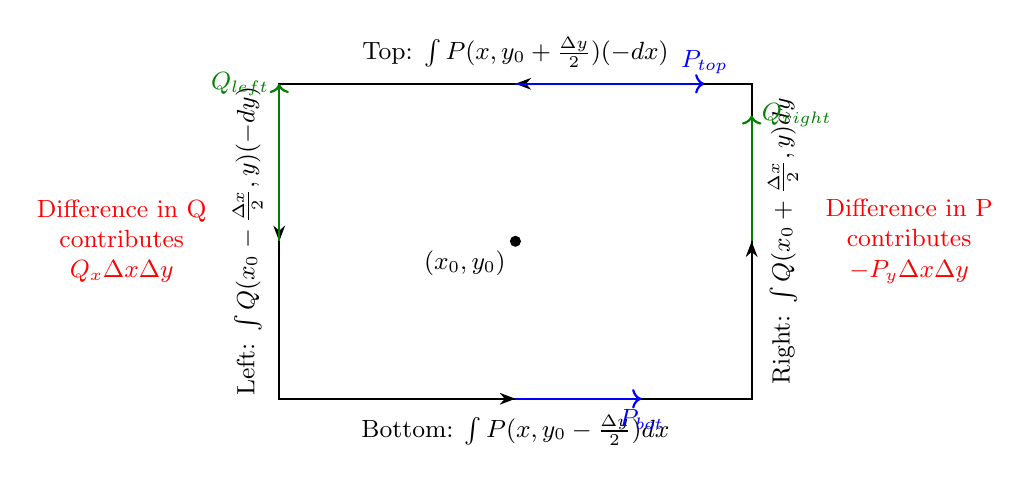
\begin{tikzpicture}[scale=2, font=\small]
			% Draw rectangle and center point
			\draw[thick] (-1.5,-1) rectangle (1.5,1);
			\fill (0,0) circle (1pt) node[below left] {$(x_0, y_0)$};
			
			% Add arrows for CCW circulation path
			\draw[-{Stealth[length=2mm]}] (-1.5, -1) -- (0, -1);
			\draw[-{Stealth[length=2mm]}] (1.5, -1) -- (1.5, 0);
			\draw[-{Stealth[length=2mm]}] (1.5, 1) -- (0, 1);
			\draw[-{Stealth[length=2mm]}] (-1.5, 1) -- (-1.5, 0);
			
			% Label path segments
			\node at (0, -1.2) {Bottom: $\int P(x, y_0-\frac{\Delta y}{2}) dx$};
			\node at (0, 1.2) {Top: $\int P(x, y_0+\frac{\Delta y}{2}) (-dx)$};
			\node[rotate=90] at (1.7, 0) {Right: $\int Q(x_0+\frac{\Delta x}{2}, y) dy$};
			\node[rotate=90] at (-1.7, 0) {Left: $\int Q(x_0-\frac{\Delta x}{2}, y) (-dy)$};
			
			% Illustrate change in P and Q
			\draw[->, thick, blue] (0, 1) -- (1.2, 1) node[above] {$P_{top}$};
			\draw[->, thick, blue] (0, -1) -- (0.8, -1) node[below] {$P_{bot}$};
			\node[red, align=center] at (2.5, 0) {Difference in P\\contributes\\$-P_y \Delta x \Delta y$};
			
			\draw[->, thick, green!50!black] (1.5, 0) -- (1.5, 0.8) node[right] {$Q_{right}$};
			\draw[->, thick, green!50!black] (-1.5, 0) -- (-1.5, 1.0) node[left] {$Q_{left}$};
			\node[red, align=center] at (-2.5, 0) {Difference in Q\\contributes\\$Q_x \Delta x \Delta y$};
		\end{tikzpicture}
		\caption{Circulation around an infinitesimal rectangle. The net circulation arises from the difference in the vector field components on opposite sides.}
		\label{fig:local_circ}
	\end{figure}
	
	Taylor expand \(P,Q\) to first order along each edge and keep first-order terms. One obtains
	\[
	\oint_{\partial R}\vec F\cdot d\vec r
	\approx \left(\frac{\partial Q}{\partial x}(x_0,y_0)-\frac{\partial P}{\partial y}(x_0,y_0)\right)\,\Delta x\,\Delta y.
	\]
	Dividing by the area \(\Delta A=\Delta x\,\Delta y\) and shrinking the rectangle,
	\[
	\lim_{\Delta A\to 0}\frac{1}{\Delta A}\oint_{\partial R}\vec F\cdot d\vec r
	= \frac{\partial Q}{\partial x}(x_0,y_0)-\frac{\partial P}{\partial y}(x_0,y_0).
	\]
	Thus the scalar \(Q_x-P_y\) is the \emph{circulation per unit area}---the 2D curl.
	
	\section*{Green's theorem (global circulation)}
	If \(C=\partial D\) is a positively oriented simple closed curve enclosing a region \(D\),
	Green's theorem states
	\[
	\oint_{C}\vec F\cdot d\vec r
	=\iint_{D}\Big(\frac{\partial Q}{\partial x}-\frac{\partial P}{\partial y}\Big)\,dA.
	\]
	So the total circulation equals the area integral of the local circulation density.
	
	\begin{figure}[h!]
		\centering
		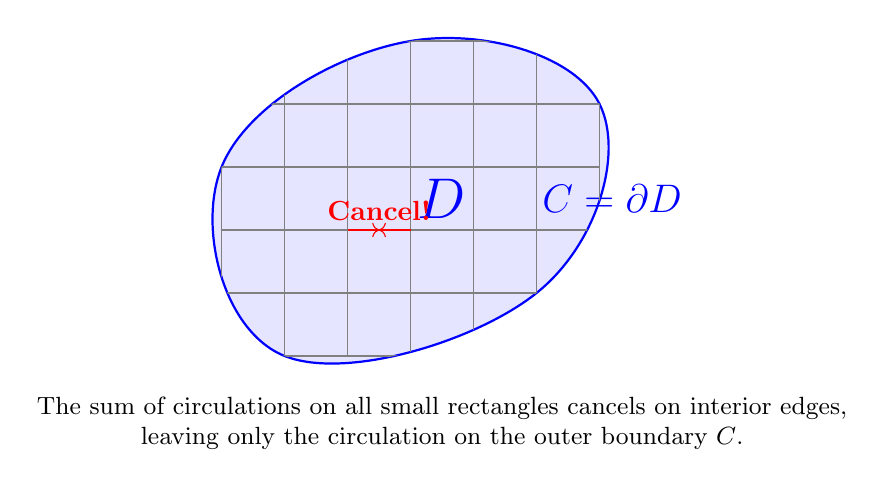
\begin{tikzpicture}[scale=0.8]
			% Draw the domain D and boundary C
			\draw[thick, blue, fill=blue!10] plot [smooth cycle, tension=0.7] coordinates {(0,0) (4,1) (5,4) (2,5) (-1,3)};
			\node[blue] at (2.5, 2.5) {\huge $D$};
			\node[blue] at (5.2, 2.5) {\Large $C = \partial D$};
			
			% Draw a grid of small rectangles inside
			\begin{scope}
				\clip plot [smooth cycle, tension=0.7] coordinates {(0,0) (4,1) (5,4) (2,5) (-1,3)};
				\draw[gray, thin] (-1,0) grid (5,5);
			\end{scope}
			
			% Show cancellation of interior paths
			\begin{scope}[decoration={
					markings,
					mark=at position 0.5 with {\arrow{>}}}
				]
				% Two adjacent rectangles
				\draw[red, postaction={decorate}] (1,2) -- (2,2);
				\draw[red, postaction={decorate}] (2,2) -- (1,2);
				\node[red, font=\bfseries] at (1.5, 2.3) {Cancel!};
			\end{scope}
			
			\node[align=center, below, font=\small] at (2.5, -0.5)
			{The sum of circulations on all small rectangles cancels on interior edges, \\ leaving only the circulation on the outer boundary $C$.};
		\end{tikzpicture}
		\caption{Green's theorem intuition: Total circulation is the sum of local circulations.}
		\label{fig:greens_thm}
	\end{figure}
	
	\section*{Example 1: Rigid rotation and angular velocity}
	Consider the rigid rotation field with angular speed \(\omega\):
	\[
	\vec F(x,y)=\langle -\omega y,\ \omega x\rangle.
	\]
	Then
	\[
	\frac{\partial Q}{\partial x}=\omega,\qquad \frac{\partial P}{\partial y}=-\omega
	\quad\Rightarrow\quad
	\operatorname{curl}\vec F = Q_x - P_y = 2\omega.
	\]
	This shows curl equals twice the angular velocity. For a circle of radius \(R\),
	parametrize \(r(t)=(R\cos t,R\sin t)\), \(dr=(-R\sin t,R\cos t)\,dt\). Then
	\[
	\oint \vec F\cdot d\vec r
	=\int_0^{2\pi}\omega R^2\,dt
	=2\pi\omega R^2.
	\]
	Meanwhile, \(\iint_{D}(2\omega)\,dA=2\omega \cdot \pi R^2=2\pi\omega R^2\), agreeing with Green's theorem.
	
	\begin{figure}[h!]
		\centering
		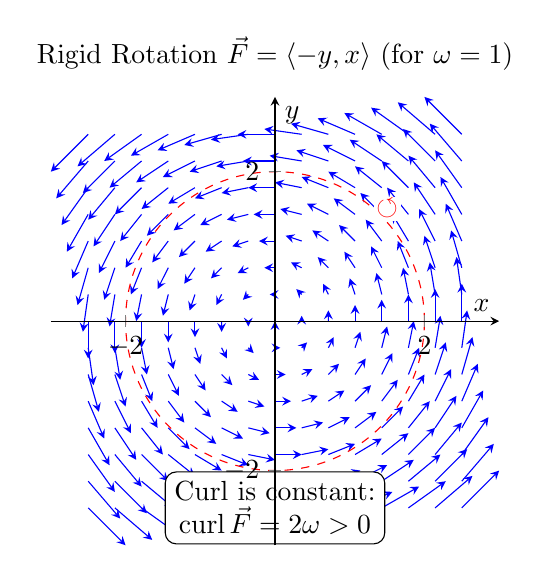
\begin{tikzpicture}
			\begin{axis}[
				title={Rigid Rotation $\vec F=\langle -y, x\rangle$ (for $\omega=1$)},
				axis equal image, view={0}{90},
				xmin=-3, xmax=3, ymin=-3, ymax=3,
				axis lines=middle, xlabel=$x$, ylabel=$y$
				]
				\addplot3[
				blue,
				quiver={
					u={-y}, v={x},
					scale arrows=0.2,
				},
				-stealth,
				domain=-2.5:2.5, domain y=-2.5:2.5,
				samples=15
				] {0};
				
				% Draw a circle and paddle wheel
				\draw[red, dashed] (axis cs:0,0) circle (2);
				\node[red, fill=white, inner sep=1pt, anchor=center] at (axis cs:1.5,1.5) {$\circlearrowleft$};
				
				\node[align=center, fill=white, draw, rounded corners] at (axis cs:0, -2.5) {Curl is constant: \\ $\operatorname{curl}\vec F = 2\omega > 0$};
			\end{axis}
		\end{tikzpicture}
		\caption{A rigid rotation field has a constant, positive curl, indicating a uniform counter-clockwise rotation at every point.}
		\label{fig:rigid_rotation}
	\end{figure}
	
	
	\section*{Example 2: Curl-free but not conservative (topology matters)}
	On \(\mathbb{R}^2\setminus\{(0,0)\}\), define
	\[
	\vec F(x,y)=\Big\langle -\frac{y}{x^2+y^2},\ \frac{x}{x^2+y^2}\Big\rangle.
	\]
	A direct calculation shows \(Q_x-P_y=0\) wherever defined (curl-free). However, the circulation
	around the unit circle is
	\[
	\oint \vec F\cdot d\vec r=2\pi\neq 0.
	\]
	Hence there is no global potential function; the puncture creates a topological obstruction.
	This illustrates that \(\operatorname{curl}\vec F=0\) captures \emph{local} rotation, while global
	circulation can persist in domains with holes.
	
%\begin{tikzpicture}
%	\begin{axis}[
%		title={Punctured Plane Field $\vec F=\langle -y/r^2, x/r^2\rangle$},
%		axis equal image, view={0}{90},
%		xmin=-3, xmax=3, ymin=-3, ymax=3,
%		axis lines=middle, xlabel=$x$, ylabel=$y$,
%		unbounded coords=discard  % <-- This is the fix
%		]
%		\addplot3[
%		blue,
%		quiver={
%			u={-y/(x^2+y^2)}, v={x/(x^2+y^2)},
%			scale arrows=0.5,
%		},
%		-stealth,
%		domain=-2.5:2.5, domain y=-2.5:2.5,
%		samples=15
%		] {0};
%		
%		% ... rest of your annotations ...
%		
%	\end{axis}
%\end{tikzpicture}
	
	\section*{Summary checklist}
	\begin{itemize}[nosep]
		\item \(Q_x-P_y\) is the infinitesimal (per-area) circulation density.
		\item Green's theorem sums local curl to give total circulation.
		\item Rigid rotation: \(\operatorname{curl}=2\omega\) (twice angular velocity).
		\item Curl \(=0\) can still have nonzero loop integrals if the domain has holes.
	\end{itemize}
	
\end{document}